\documentclass[12pt, a4paper]{article}
%%import package named techno
\usepackage{techno}
\usepackage[export]{adjustbox}
\usepackage{wrapfig}
\DeclareSymbolFont{matha}{OML}{txmi}{m}{it}% txfonts
\DeclareMathSymbol{\varv}{\mathord}{matha}{118}
\usepackage{tkz-tab}
\usepackage{chemfig}
\newtheorem*{exc*}{\kml រូបមន្ត}
\tcolorboxenvironment{exc*}{colback=cyan!5!white,colframe=blue}
\usepackage{tikz}
\usepackage[b]{esvect}    % For \vv
\usepackage{tikz}         % For arrow and dots in \xvec
\usepackage{circuitikz}
\usepackage{graphicx}
\graphicspath{ {./images/} }
%សរសេរគីមីវិទ្យា
%\usepackage[version=3]{mhchem}
%\usepackage{mathpazo}% change math font
%\usepackage[no-math]{fontspec}% font specfication
\everymath{\protect\displaystyle\protect\color{black}}
\begin{document}
\maketitle\koc
\begin{enumerate}[I]
	\item {\kml ទ្រឹស្តីសុីនេទិចនៃឧស្ម័ន}
	\begin{multicols}{2}
		\begin{enumerate}[m]
			\item ម៉ូលេគុលឧស្ម័នទាំងអស់ធ្វើចលនាឥតឈប់ឈរ និងគ្មានសណ្តាប់ធ្នាប់។
			\item គ្រប់ការទង្គិចរបស់ម៉ូលេគុលជាទង្គិចខ្ទាត។
			\item គេសន្មតថាម៉ូលេគុលនីមួយៗមានល្បឿនថេរជានិច្ច និងអាចអនុវត្តច្បាប់ញ៉ូតុនបានគ្រប់ពេល។
			\item គេចាត់ទុកម៉ូលេគុលឧស្ម័នជាចំណុចរូបធាតុ ព្រោះវិមាត្ររបស់ម៉ូលេគុលនីមួយៗតូចធៀបនឹងលំហអន្តរម៉ូលេគុល។
			\item ថាមពលសុីនេទិចមធ្យមនៃម៉ូលេគុលសមាមាត្រនឹងសីតុណ្ហភាព។
		\end{enumerate}
		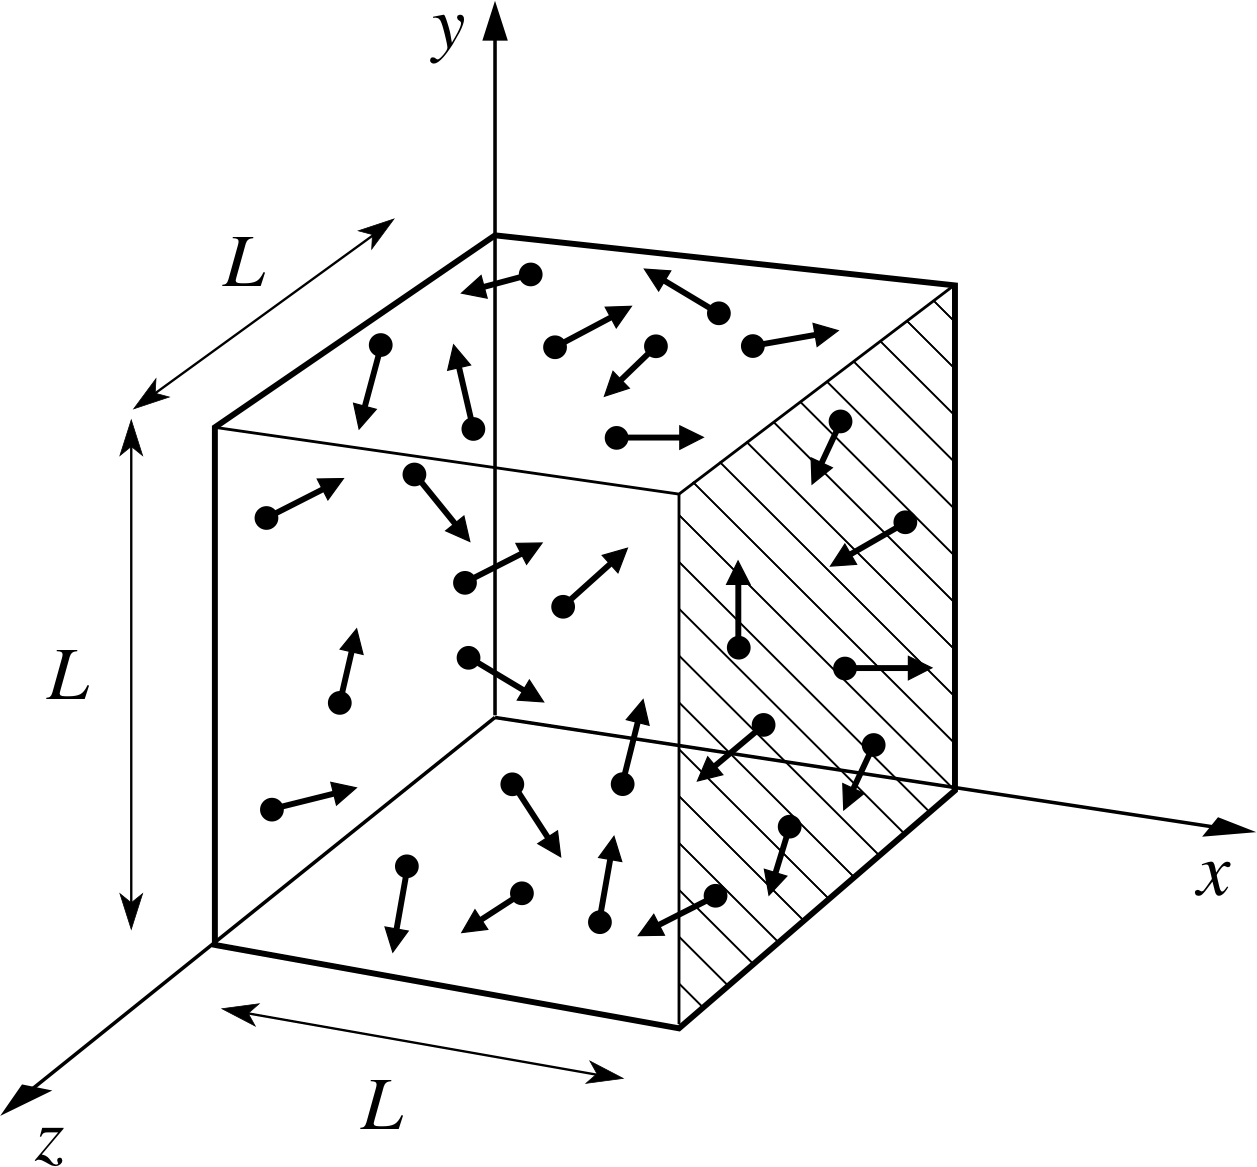
\includegraphics[scale=1]{01}
	\end{multicols}
	\item {\kml សម្ពាធក្នុងទ្រឹស្តីសុីនេទិចនៃឧស្ម័នៈ}\\
	\quad យើងសិក្សាចលនាម៉ូលេគុលក្នុងធុងមួយ។ យើងបានសម្ពាធដែលសង្តត់លើផ្ទៃធុងគឺជាកម្លាំងទង្គិចរបស់ចលនាម៉ូលេគុល
	\begin{align*}
		\text{យើងបាន}\quad :&\quad P=\frac{F}{A}\quad \text{ដោយ}: \quad F=m\frac{\Delta \upsilon_{x}}{\Delta t}=\frac{m\times2\upsilon_{x}}{\frac{2L}{\upsilon_{x}}}=\frac{m\upsilon^{2}_{x}}{L}\\
		\text{យើងបាន}\quad :&\quad P=\frac{m\upsilon^{2}_{x}}{AL}=\frac{m\upsilon^{2}_{x}}{V}\\
		\text{តែ}\quad :&\quad \left(\upsilon^{2}\right)_{av}=\left(\upsilon^{2}_{x}\right)_{av}+\left(\upsilon^{2}_{y}\right)_{av}+\left(\upsilon^{2}_{z}\right)_{av}=3\left(\upsilon^{2}_{x}\right)_{av}\\\text{ដែល}\quad & \left(\upsilon=\upsilon_{x}=\upsilon_{y}=\upsilon_{z}=\text{ថេរ}\right)\\
		\text{នាំឲ្យ}\quad :&\quad \left(\upsilon^2_{x}\right)_{av}=\frac{1}{3}\left(\upsilon^2\right)_{av}\\
		\text{យើងបានសម្ពាធលើផ្ទៃខាងនីមួយៗ កំណត់ដោយៈ}\quad :&\quad P=\frac{1}{3}\times\frac{m}{V}\left(\upsilon^{2}\right)_{av}\quad \text{ឬ}\quad P=\frac{1}{3}\rho\left(\upsilon^{2}\right)_{av}\\
		\text{ដែល}\quad :&\quad \rho =\frac{m}{V}\left(\text{ម៉ាសមាឌ}\right)\\
		\text{ម្យ៉ាងទៀត}\quad :&\quad m=m_{0}N\\
		\text{យើងបាន}\quad :&\quad P=\frac{1}{3}\times\frac{Nm_{0}}{V}\left(\upsilon^{2}\right)_{av}=\frac{2N}{3V}\times\frac{1}{2}m_{0}\left(\upsilon^2\right)_{av}\\
		\text{ដូចនេះ}\quad :&\quad P=\frac{2}{3}\times\frac{N}{V}K_{av}
	\end{align*}
	\item {\kml ថាមពលសុីនេទិច និងសីតុណ្ហភាព}
	\begin{enumerate}[m]
		\item {\kml សមីការភាពនៃឧស្ម័នបរិសុទ្ធៈ} តាមពិសោធន៍បង្ហាញថាៈ
		\begin{itemize}
			\begin{multicols}{2}
				\item សម្ពាធសមាមាត្រនឹងសីតុណ្ហភាព\quad : \quad $P\sim T$
				\item សម្ពាធសមាមាត្រនឹងចំនួនម៉ូលេគុល\quad : \quad $P\sim N$
				\item សម្ពាធច្រាសសមាមាត្រនឹងមាឌ\quad : \quad $P\sim\frac{1}{V}$
			\end{multicols}
		\end{itemize}
	\begin{align*}
		\text{យើងបាន}\quad :& \quad P\sim \frac{NT}{V}\quad \text{ឬ}\quad P=k_{B}\frac{NT}{V}\quad \text{នោះ}\quad PV=Nk_{B}T\quad\text{ដែល}\quad k_{B}=1.38\times10^{-23}J/K\left(\text{ថេរបុលស្មាន់}\right)\\
		\text{តែ}\quad :&\quad N=nN_{A}\quad \text{នោះ}\quad PV=nk_{B}N_{A}T\\
		\text{តាង}\quad :&\quad R=k_{B}N_{A}\quad\text{ដែល}\quad N_{A}=6.02\times10^{23}\text{ម៉ូលេគុល}/mol\left(\text{ចំនួនអាវ៉ូកាដ្រូ}\right)\\
		\text{ដូចនេះ}\quad :&\quad PV=k_{B}NT=nRT
	\end{align*}
	\item {\kml សមីការបម្រែបម្រួលភាពនៃឧស្ម័នបរិសុទ្ធៈ} បើឧស្ម័នប្រែប្រួលភាព ពីភាពដើម $1$ ទៅភាពស្រេច $2$ យើងបានៈ
	\begin{itemize}
		\begin{multicols}{2}
			\item នៅភាពដើម $1$: $P_{1}V_{1}=nRT_{1}$ ឬ $\frac{P_{1}V_{1}}{T_{1}}=nR$
			\item នៅភាពស្រេច $2$: $P_{2}V_{2}=nRT_{2}$ ឬ $\frac{P_{2}V_{2}}{T_{2}}=nR$
		\end{multicols}
	\end{itemize}
	\begin{align*}
		\text{យើងបាន}\quad :&\quad \frac{P_1V_1}{T_1}=\frac{P_2V_2}{T_2}=nR=\text{ថេរ}\\
		\text{ច្បាប់ប៊យ-ម៉ារ្យ៉ូត}\quad :&\quad P_{1}V_{1}=P_{2}V_{2}\quad \left(\text{សីតុណ្ហភាពថេរ} T_{1}=T_{2}\right)\\
		\text{ច្បាប់សាល}\quad :&\quad \frac{P_1}{T_1}=\frac{P_2}{T_2}\quad \left(\text{មាឌថេរ} V_{1}=V_{2}\right)\\
		\text{ច្បាប់កេលុយសាក់}\quad :&\quad \frac{P_1V_1}{T_1}=\frac{P_2V_2}{T_2}\\
	\end{align*}
	\item {\kml ថាមពលសុីនេទិច និងសីតុណ្ហភាពៈ}
		\begin{enumerate}[k]
			\item {\kml តម្លៃថាមពលសុីនេទិចមធ្យមនៃម៉ូលេគុលឧស្ម័នៈ}
			\begin{align*}
			\text{តាមសម្រាយបញ្ជាក់ខាងលើ}\quad :&\quad P=\frac{2}{3}\times\frac{N}{V}K_{av}\quad \text{យើងបានៈ}\quad PV=\frac{2}{3}NK_{av}\\
			\text{នាំឲ្យ}\quad :&\quad K_{av}=\frac{3}{2}\times\frac{PV}{N}=\frac{3}{2}k_{B}T \quad\text{ព្រោះ}\quad \frac{PV}{N}=k_{B}T\\
			\text{ដូចនេះ តម្លៃថាមពលសុីនេទិចមធ្យមនៃម៉ូលេគុលឧស្ម័នគឺៈ}\quad :& \quad K_{av}=\frac{3}{2}k_{B}T=\frac{3}{2}\left(\frac{PV}{N}\right)
			\end{align*}
			\item {\kml តម្លៃថាមពលសុីនេទិចសរុបនៃម៉ូលេគុលឧស្ម័នៈ}
			\begin{align*}
				\text{យើងមាន}\quad :&\quad K_{av}=\frac{3}{2}k_{B}T\\
				\text{នាំឲ្យ}\quad :&\quad K=N\times K_{av}=\frac{3}{2}Nk_{B}T=\frac{3}{2}nRT\\
				\text{ដូចនេះ តម្លៃថាមពលសុីនេទិចសរុបនៃម៉ូលេគុលឧស្ម័នគឺៈ}\quad :& \quad K=\frac{3}{2}Nk_{B}T=\frac{3}{2}nRT
			\end{align*}
		\end{enumerate}
		\item {\kml ល្បឿនប្ញសការេនៃការេល្បឿនមធ្យមៈ}
		\begin{align*}
			\text{យើងមាន}\quad :& \quad K_{av}=\frac{3}{2}k_{B}T=\frac{1}{2}m_{0}\left(\upsilon^{2}\right)_{av}\\
			\text{នាំឲ្យ}\quad :&\quad \sqrt{\left(\upsilon^{2}\right)_{av}}=\sqrt{\frac{3k_{B}T}{m_{0}}}\\
			\text{តាង}\quad :& \quad \upsilon_{rms}=\sqrt{\left(\upsilon^{2}\right)_{av}}=\sqrt{\frac{3k_{B}T}{m_{0}}}=\sqrt{\frac{3RT}{M}}\quad \left(\text{\en Root Means Square}\right)\\
			\text{ដូចនេះ ល្បឿនប្ញសការេនៃការេល្បឿនមធ្យមគឺៈ}\quad :& \quad \upsilon_{rms}=\sqrt{\frac{3k_{B}T}{m_{0}}}=\sqrt{\frac{3RT}{M}}
		\end{align*}
	\end{enumerate}
\begin{itemize}
	\item[$\ast$] {\kml ចំណាំៈ}
	\begin{enumerate}[m]
		\item ល្បឿនមធ្យមៈ $\upsilon_{av}=\frac{\upsilon_{1}+\upsilon_{2}+\upsilon_{3}+\cdots+\upsilon_{N}}{N}$\quad ដែល\quad $\upsilon_{av}$ គិតជា $m/s$\\
		$\left(\upsilon_{av}\right)^2=\left(\overline{\upsilon}\right)^2=\left(\frac{\upsilon_1+\upsilon_2+\upsilon_3+\cdots+\upsilon_{N}}{N}\right)^2$ ល្បឿនមធ្យមលើកជាការេ គិតជា $m/s$\\
		$\left(\upsilon^2\right)_{av}=\upsilon^2_{rms}=\frac{\upsilon^2_1+\upsilon^2_2+\upsilon^2_3+\cdots+\upsilon^2_{N}}{N}$ តម្លៃមធ្យមនៃការេល្បឿន​ គិតជា $m/s$\\
		\item ល្បឿនប្ញសការេនៃការេល្បឿនមធ្យមៈ $\upsilon_{rms}=\sqrt{\left(\upsilon^2\right)_{av}}=\sqrt{\frac{\upsilon^2_{1}+\upsilon^2_{2}+\upsilon^2_{3}+ \cdots+\upsilon^2_{N}}{N}}$\quad ដែល\quad $\upsilon_{rms}$ គិតជា $m/s$\\
		$\upsilon^2_{rms}=\left(\upsilon^2\right)_{av}$
		\item ម៉ាសមាឌ ឬដង់សុីតេមាឌនៃឧស្ម័នៈ $\rho=\frac{m}{V}=\frac{m_{0}N}{V}$\quad ដែល\quad $\rho$ គិតជា $\left(kg/m^3\right)$\\ $m$ ជាម៉ាសឧស្ម័ន គិតជា $\left(kg\right)$\\ $m_{0}$ ម៉ាសមូលេគុល គិតជា $\left(kg\right)$ 
		\\ $V$ មាឌឧស្ម័ន គិតជា $\left(m^3\right)$
		\item ចំនួនម៉ូលៈ $n=\frac{m}{M}=\frac{N}{N_{A}}=\frac{V}{V_{mol}}$\quad ដែល\quad $M$ ម៉ាសម៉ូលគិតជា $\left(kg\right)$\\
		$N$ ចំនួនម៉ូលេគុលសរុប\\
		$V_{mol}$ ជាមាឌឧស្ម័នក្នុងមួយម៉ូល $\left(m^3/mol\right)$\\
		$V$ មាឌឧស្ម័ន $\left(m^3\right)$
		\item ចំនូនម៉ូលេគុលសរុបនៃឧស្ម័នៈ $N=\frac{m}{m_{0}}=nN_{A}=\frac{m}{M}\times N_{A}$ ដែល $n$ ចំនួនម៉ូល​ គិតជា $\left(mol\right)$
		\item មាឌម៉ូលនៃឧស្ម័នក្នុងលក្ខខ័ណ្ឌគំរូដែលមានសម្ពាធ $P_{0}=1atm$ និងសីតុណ្ហភាព $T=273K$ គឺៈ $V_{mol}=22.4\times10^{-3}m^3/mol$
		\item ល្បឿននៃចលនាត្រង់ស្មើៈ(បម្លាស់ទី=ល្បឿន$\times$ រយៈពេល) $x=\upsilon\times\Delta t$
	\end{enumerate}
\end{itemize}
\end{enumerate}
\begin{center}
	\sffamily\color{blue}
	\huge ចប់ដោយសង្ខេប!
\end{center}
\newpage
\begin{exc*}
	ការដែល
\end{exc*}
\newpage
\begin{center}
	{\kml \large ច្បាប់ទីមួយទែម៉ូឌីណាមិច}\\
	{\enb \large The First Law of Thermodynamics}
\end{center}
\begin{enumerate}[I]
	\item {\kml ប្រព័ន្ធទែម៉ូឌីណាមិចៈ}
		\begin{enumerate}[m]
			\item {\kml ប្រព័ន្ធៈ} គឺជាវត្ថុ ឬសំណុំវត្ថុដែលយើងលើកមកសិក្សា ដោយធៀបទៅនឹងវត្ថុដ៏ទៃផ្សេងទៀត។\\(វត្ថុដ៏ទៃផ្សេងទៀតនោះ យើងហៅថាៈ មជ្ឈដ្ឋានក្រៅ)
			\item {\kml ភាពនៃប្រព័ន្ធៈ} គឺជាសំណុំលេខដែលវាស់ទំហំរូបវិទ្យា ដើម្បីសម្គាល់ប្រព័ន្ធនៅខណៈណាមួយ មានមាឌ សម្ពាធ និងសីតុណ្ហភាពជាអថេរសម្គាល់ភាពនៃប្រព័ន្ធ ។
			\item {\kml បម្លែងទែម៉ូឌីណាមិចៈ} ប្រព័ន្ធមួយទទួលបម្លែងទែម៉ូឌីណាមិច កាលណាវាផ្លាស់ប្តូរភាព ដោយប្តូរតែ កម្មន្ត និងកម្តៅ ជាមួយមជ្ឈដ្ឋានក្រៅប៉ុណ្ណោះ។ គេចែកបម្លែងទែម៉ូឌីណាមិចជាពីរគឺ បម្លែងចំហ និងបម្លែងបិទ។
			\begin{itemize}
				\item [$\ast$] បម្លែងចំហ-បម្លែងបិទៈ ពេលប្រព័ន្ធមួយទទួលបម្លែងទែម៉ូឌីណាមិចៈ
				\begin{itemize}
					\item បើភាពដើម និងភាពស្រេចនៃប្រព័ន្ធមួយ ខុសគ្នា នោះគេថាប្រព័ន្ធទទួលរងនូវបម្លែចំហ។
					\item បើភាពដើម និងភាពស្រេចនៃប្រព័ន្ធមួយ ដូចគ្នា នោះគេថាប្រព័ន្ធទទួលរងនូវបម្លែងបិទ។
				\end{itemize}
			\end{itemize}
			\item {\kml ប្រព័ន្ធទែម៉ូឌីណាមិចៈ} គឺជាប្រព័ន្ធដែលទទួល បម្លែងទែម៉ូឌីណាមិចដោយមានការផ្លាស់ប្តូរភាពដើម និងភាពស្រេចតាមដំណើរប្រព្រឹត្តទៅខុសៗគ្នា។
			\begin{itemize}
				\item [$\ast$] សមីការប្រែប្រួលភាពនៃឧស្ម័នបរិសុទ្ធៈ $\frac{P_1V_1}{T_1}=\frac{P_2V_2}{T_2}=nR=const$(ថេរ)\\
				ដែលភាពដើម $P_1,V_1$ សម្ពាធ និងមាឌឧស្ម័ននៅសីតុណ្ហភាព $T_1$ និង ភាពស្រេច $P_2,V_2$ សម្ពាធ និងមាឌឧស្ម័ននៅសីតុណ្ហភាព $T_2$ មាឌគិតជា $m^3$ សីតុណ្ហភាពគិតជា $K$ និងសម្ពាធគិតជា $Pa$\quad($V_1, V_2$ អាចគិតជា $L$ ក៏បាន)។
			\end{itemize}
		\end{enumerate}
	\item {\kml កម្មន្តបំពេញក្នុងពេលបម្រែបម្រួលមាឌៈ}
	\begin{enumerate}[m]
		\item {\kml ករណីសម្ពាធថេរ(លំនាំអុីសូបារ):} $P_1=P_2=$ ថេរ
	\end{enumerate}
\end{enumerate}
\begin{center}
	\sffamily\color{blue}
	\huge ចប់ដោយសង្ខេប!
\end{center}
\end{document}